\section{Planning expectations management}
\begin{itemize}
    \item Claude Debussy and Mozart are quoted as saying that music is the silence between the notes.
    \item To many respects PM has a component of what is seen and what is seen. A project is as much the things that aren't seen as the things that are.
    \item A good PM will have a sense of the expectations, assumptions and risks of a project.
\end{itemize}

\subsection{Expectations}
\begin{itemize}
    \item Take into account that all stakeholders are different and will have different expectations.
    \item Some people will be satisfied and others will be disapointed.
    \item Expectation: is the psycological picture we create in our heads for a future event. If you give a person room to imagine and make their own expectations there will be a tendency to over expect or under expect.
    \item Expectations vary person to person. Same with projects, the stakeholders need to be in the same page as the PM in order to manage these expectations.
    \item Getting everyone on the same page is done during the scope definition with the stakeholders. The PM must need to communicate what should be expected. Some questions you could ask are:
        \begin{itemize}
            \item How do you thing the final product of the project will be useful to the organization?
            \item Do you believe soething can be added to significantly improve the result?
            \item Do you agree with the way the scope is described in the project documents?
            \item Many many more questions, the more the better expectation handling you can do.
        \end{itemize}
    
    \item Managing the stakeholder's expectations is super important because these eventually become the acceptance criteria of the project.
    \item A successful project has the following characteristics:
        \begin{itemize}
            \item Keep all stakeholders up to date through the scope phase.
            \item Keep in constant communications with the stakeholders as any changes occur.
            \item Eliminate any stakeholders' disappointments.
        \end{itemize}
\end{itemize}

%%%%%%%%%%%%%%%%%%%%%%%%%%%%%%%%%%%%%%%%%%%%%%%%%%%%%%
\section{How to control assumptions}
\begin{itemize}
    \item An assumption is when something is believed to be true when there is no definite proof.
    \item We must always assume that in a project there are areas that we cannot 100\% be certain of.
    \item We cannot be 100\% sure that all team members will be as productive as they usually are, but we have to assume they will.
    \item The more past data (historic data) there are about past projects and members the better the assumptions.
\end{itemize}

%%%%%%%%%%%%%%%%%%%%%%%%%%%%%%%%%%%%%%%%%%%%%%%%%%%%%%
\section{Planning Risk management}
\begin{itemize}
    \item Proper risk management can save a project from total failure.
    \item PM is looking to succeed can follow the following steps:
        \begin{enumerate}
            \item Identify all the risks in a risk log. Not a straight forward process. You must involve the team and stakeholders in risk assesment. A risk log may look like this:
                \begin{figure}[H]
                    \centering
                    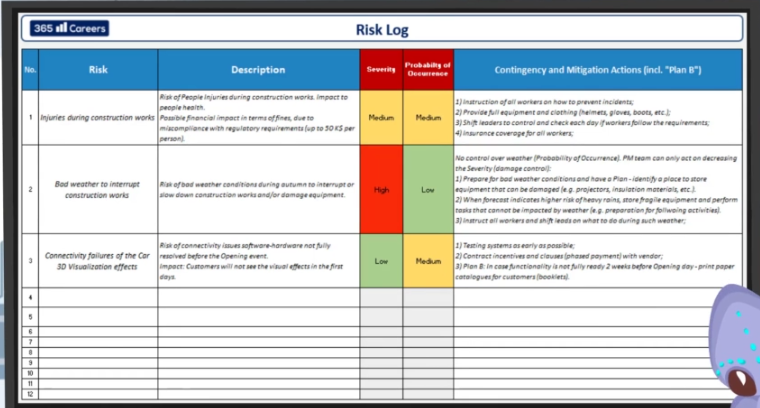
\includegraphics[width=\width\textwidth]{./figs/20221027155606.png}
                    %\caption{}
                \end{figure}
            
            \item Analyse risks:
                \begin{itemize}
                    \item Review 2 dimensions: 1. how bad can it get if the event happens. 2. How likely it is that the event actually happens. In other words the severity and the probability of occurance.
                    \item The severity refers to the impact the event would have on the scope, budget or timeline. We record it in a scale, it can be a scale such as high, medium, and low, or you can measure it in financial losses too. The scale can be decided according to each project and what risks it entails.
                    \item The probability of occurance is how likely an event will occur. You can choose which scale to use (high, low, medium, percentage, etc).
                \end{itemize}
        \end{enumerate}
\end{itemize}

%%%%%%%%%%%%%%%%%%%%%%%%%%%%%%%%%%%%%%%%%%%%%%%%%%%%%%
\section{Building a Risk log}
\begin{itemize}
    \item When faced with a risk do:
        \begin{enumerate}
            \item Mitigation: Change something in advance to lessen or eliminate the risk.
            \item Contigency: Create a plan B in case the risk becomes reality.
        \end{enumerate}
    
    \item Mitigation: eliminate and mitigating the risk you can plan strategies. 
    \item Contingency: If eliminating the risk is not possible or not worth the extra costs, you can aim to reduce the severity.
    \item These methods can be combined.
    \item Contingency planning: unless you have elminated a risk completely then a plan B is always a good idea.
        \begin{figure}[H]
            \centering
            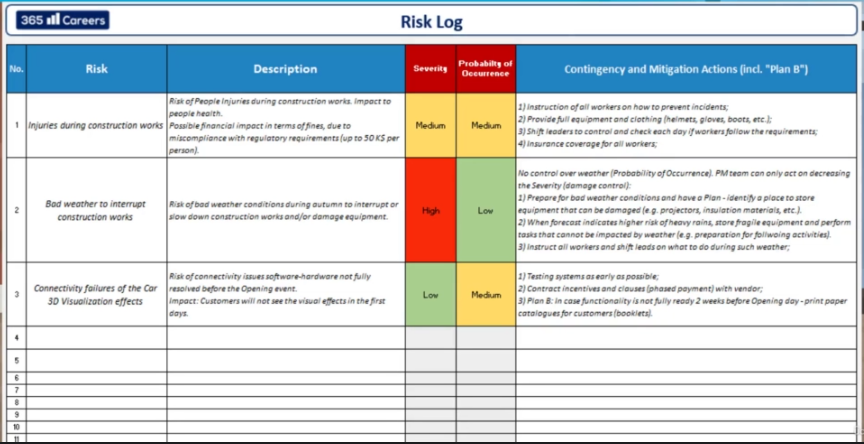
\includegraphics[width=\width\textwidth]{./figs/20221027161657.png}
            %\caption{}
        \end{figure}
    
    \item A risk log is a living document that must be constantly updated.
    \item Risks are often identified through communication with stakeholders.
\end{itemize}

